% Nama Kelompok : Procces address space
% Kelas : D4 TI 1A
% 1. Dwi Yulianingsih
% 2. Habib Abdul Rasyid
% 3. Kukuh Yunaswara
% 4. Felix Setiawan Lase
% 5. Muhammad Dzihan Albana

\section {Proses Address Space}

\subsection {A. Konsep dasar memori}

\begin{figure}[ht]
\centerline{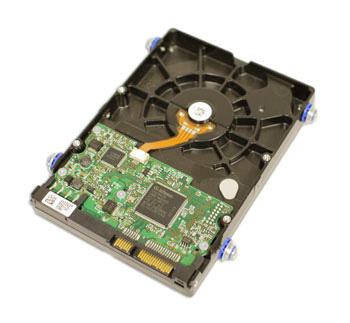
\includegraphics[width=0.5\textwidth]{figures/drive.jpg}}
\caption{Hard Drive}
\label{Drive}
\end{figure}

Memori adalah sebagai suatu pusat dari operasi yang pada setiap komputer modern , memori berfungsi untuk tempat penyimpan sebuah informasi dan harus diatur dan dijaga sebaik mungkin . memori adalah array besar dari word atau byte yang bisa disebut alamat CPU untuk mengambil instruksi instruksi dari sebuah memory, perangkat tersebut mengambil perintah-perintah pada memori menurut nilai dari penghitung program  program.
Sedangkan manajemen memori adalah kegiatan untuk mengatur memori komputer. Proses ini akan menyediakan cara untuk mengalokasikan memori untuk memproses atas sebuah  permintaan mereka, membebaskannya untuk digunakan kembali ketika tidak lagi diperlukan dan mempertahankan alokasi ruang memori untuk proses tersebut. Manajemen memori utama sangat penting untuk sistem komputer  penting untuk mengolah dan menginput fasilitas atau keluaran secara efisien, sehingga memori dapat ditampung sebanyak mungkin proses dan dalam upaya pemogram atau proses tidak terbatas kapasitas memori fisik dalam sistem komputer (Eko, 2009).
Memory manager merupakan suatu bagian dari sistem operasi yang sangat berperan dalam menentukan proses-proses yang ditempatkan pada antrian.
Jenis jenis Memori seperti memori kerja, ROM, PROM, EPROM, EEPROM, RAM, Memori cache, memori yang dapat didukung Floppy hard drive dan cd.
Jenis jenis Alamat pada memori memiliki 4 yaitu alamat memori , alamat memori relative , Hubungan antara alamat multak dan alamat relative dan Jenis memori dan alamat memori .
Isi Memori ada beberapa bagian yaitu Sistem bahasa peñata olahan , Sistem Utilitas, Inti Sistem Operasi , Pengendali alat (device drivers) dan File pemakai.
Fungsi dari manajemen memori dibagi menjadi 4 yaitu mengelola informasi yang digunakan dan tidak digunakan , mengalokasikan memori ke proses yang membutuhkan , mengelokasikan memori dari proses setelah selesai dan mengelola swapping atau paging antara memori utama dengan disk.\cite{giuffrida2012enhanced}

\subsection {Jenis-Jenis Yang Ada di Manajemen Memori}
Manajemen Memori umumnya digunakan untuk monoprogramming
Ketika itu sebuah program komputer yang hanya berjalan satu jenis maka selama proses berlangsung itu akan dikatakan bahwa mode kerja komputer adalah monoprogramming. Selama waktu itu komputer juga berfungsi maka memori dalam RAM sepenuhnya dikendalikan oleh program program.
Sistem operasi memberikan sebuah  tanggapan terhadap manajemen memori utama untuk aktivitas-aktivitas sepertii 

\begin{itemize}

\item Merawat dan memelihara  memori yang sedang digunakan dan dari yang menggunakan.

\item Memutuskan proses-proses mana saja yang harus dipanggil kememori jika masih ada ruang di memori.

\item Mengalokasikan dan mendelokasikan ruang memori jika diperlukan.

\end{itemize}

Jadi  RAM tidak bisa di masuki oleh program lain. Model yang  serupa ini bisa di temui pada komputer berbasis DOS.
Penempatan program di ruang penyimpanan diatur sedemikain rupa sehingga (Eko, 2009) :

\begin{enumerate}

\item BIOS selalu ada di ROM (BIOS)
\item Sistem Operasi  di bagian RAM bawah (alamat rendah)
\item Program Aplikasi di bagian RAM tengah (alamat sesudah OS terakhir)
\item Data Sementara di bagian RAM atas (alamat sesudah Aplikasi terakhir).

\end{enumerate}

jika sistem operasi telah selesai atau berhasil dimuat maka akan ada prompt muncul di layar, dan itu adalah tanda bahwa komputer siap untuk menerima program aplikasi. Masukkan disk yang berisi program aplikasi pada drive dan eksekusi disk yang aktif, sehingga program tersebut dimuat seluruhnya ke dalam RAM. Dengan demikian program aplikasi siap digunakan dengan benar. Kita melihat ketika komputer pertama kali dihidupkan maka proses yang pertama kali dibaca adalah apa yang tertulis di ROM. Setelah semua perintah di ROM BIOS selesai dibaca maka komputer meminta kita untuk memasukkan DOS ke dalam RAM-nya. Ketika DOS dibaca maka masukkan beberapa program DOS yang paling penting ke dalam RAM, seperti: COMMAND.COM dan INTERNAL COMMAND. Sementara program DOS lainnya masih tetap berada di disk dan jika kita perlu dieksekusi. Sangat berguna untuk menjaga RAM tidak penuh oleh Sistem Operasi saja.

Ketika kita bekerja dengan program aplikasi bagdi maka kita akan menghasilkan data. Data akan disimpan sementara di RAM yang tersisa. Data yang disimpan dalam RAM adalah voletile, yang berarti bahwa data hanya dapat bertahan selama daya komputer AKTIF. Untuk menyimpan kebiasaan menyimpan data ke disk dalam waktu tidak terlalu lama, misalnya setiap 5 menit.

\subsection {B. Strategi Manajemen Memori}
Strategi yang dikenal untuk mengatasi ini adalah memori virtual. Memori virtual menyebabkan sistem seolah-olah memiliki lebih banyak memori daripada keadaan memori fisik yang sebenarnya. Memori virtual tidak hanya menyediakan peningkatan komputasi, tetapi virtual memory juga memiliki kelebihan seperti:

Ruang Alamat Besar
Membuat sistem operasi tampaknya memiliki lebih banyak memori daripada kapasitas memori fisik yang ada. Dalam hal ini memori virtual memiliki ukuran yang lebih besar dari ukuran memori fisik.
Perlindungan.
Setiap proses dalam sistem memiliki ruang alamat virtual. Ruang alamat virtual dari setiap proses berbeda dari proses lainnya, sehingga apa pun yang terjadi dalam suatu proses tidak akan secara langsung mempengaruhi proses lainnya
Pemetaan Memori
Pemetaan memori digunakan untuk memetakan gambar dan file data ke dalam alamat proses. Dalam pemetaan memori, isi file akan terhubung langsung ke ruang alamat virtual dari proses

\subsection {Fair Physical Memory Allocation}
Alokasi Memori Fisik yang Adil Biasanya Digunakan dalam Manajemen Memori untuk membagi penggunaan memori fisik secara merata ke dalam setiap proses yang berjalan pada suatu sistem.

\subsection {Shared Virtual Memory}
Meskipun dalam Memori Virtual Bersama setiap proses menggunakan ruang alamat yang berbeda dari memori virtual, tetapi ada kalanya proses dihadapkan untuk berbagi penggunaan memori.\cite{kil2006address}

\subesection {C. Ruang Alamat Logika dan Fisik}
Alamat logika adalah alamat yang dihasilkan dalam CPU, juga disebut alamat virtual. Alamat fisik adalah alamat yang terlihat oleh memori. Untuk mengubah dari alamat logis ke alamat fisik perangkat keras yang disebut MMU (Memory Management Unit) diperlukan. Mengubah dari alamat logis ke alamat fisik adalah pusat manajemen memori. Alamat yang dihasilkan oleh CPU disebut alamat logis di mana alamat muncul sebagai memori uni yang disebut alamat fisik. Tujuan utama dari manajemen memori adalah konsep menempatkan ruang alamat logis ke ruang alamat fisik (Ama, 2003).

Hasil dari skema waktu gabungan dan waktu pengikatan alamat pada alamat yang logis dan alamat yang ada pada memori adalah serupa. Tetapi skema waktu pengikatan waktu untuk eksekusi alamat berbeda. dalam hal ini, alamat logis disebut alamat virtual. Himpunan semua alamat logika yang dihasilkan oleh program disebut ruang alamat logis; himpunan semua alamat fisik yang terkait dengan alamat logis disebut ruang alamat fisik.
Unit Manajemen Memori (MMU) adalah perangkat perangkat keras yang memetakan alamat virtual ke alamat fisik. Dalam skema MMU, nilai register relokasi ditambahkan ke setiap alamat yang dihasilkan oleh proses pengguna ketika dikirim ke memori.
Register dasar disebut register relokasi. Nilai register relokasi ditambahkan ke setiap alamat yang dihasilkan oleh proses pengguna ketika dikirim ke memori, misalnya, jika basisnya 14000, pengguna mencoba menempatkannya ke alamat 0 dan dipindahkan secara dinamis ke lokasi 14000. Access ke lokasi logika 346, dipetakan ke lokasi 14346. Sistem operasi MS-DOS yang masih merupakan keluarga intel 80X86 menggunakan empat register relokasi ketika memuat dan menjalankan proses.

\subsection {Multiprogramming Dengan Swapping}
manajemen memori adalah kegiatan mentransfer gambar proses antara memori utama dan disk selama eksekusi, atau dengan kata lain itu adalah pengalihan manajemen proses dari memori utama ke disk dan kembali lagi (swapping). Manajemen ini terdiri dari:
Multiprogramming Dengan Partisi Dinamis
Jumlah, lokasi, dan ukuran proses dalam memori dapat bervariasi dari waktu ke waktu secara dinamis. Kelemahan: a) Lubang memori dapat terjadi di antara partisi yang digunakan; b) mempersulit alokasi dan alokasi memori.
{Solusi}:
rongga-rongga kecil di antara blok-blok memori yang digunakan dapat diatasi dengan pemadatan memori yaitu menggabungkan semua rongga kecil menjadi satu rongga besar dengan memindahkan semua proses agar saling berdekatan.
 
Strategi Alokasi Memori
\begin{itemize}

\item First fit algorithm : memory  manager men-scan daftar untuk  menemukan lubang yang muat untuk menampung proses yg baru. Proses akan menempati lubang pertama yg ditemuinya dan cukup untuk ditempati.
\item Fit algoritma berikutnya: sama seperti fit pertama, tetapi pencarian lubang dimulai dari lubang yang ditemui dari pemindaian sebelumnya.
\item Algoritme fit terbaik: mencari lubang yang akan menghasilkan residu paling sedikit setelah proses masuk.
\item Algoritma fit terburuk: kebalikan dari fit terbaik.
\item Quick Fit algorithm: group holes dan membuat daftar mereka sendiri. Misalnya, ada daftar untuk 4K lubang, satu daftar untuk 8K, dan seterusnya.
\item Sistem Sobat: Memori dalam menumpuk di dash blok bebas ukuran 1,2,4,8,16 byte dll, hingga kapasitas memori.

\end{itemize}

Dari berbagai cara alokasi tsb. Di atas, lubang yang ditempati oleh proses akan dibagi menjadi bagian-bagian yang digunakan oleh proses dan memori yang tidak terpakai (fragmen). Munculnya memori yang tidak terpakai disebut fragmentasi. Ada dua jenis fragmen

\begin{itemize}

\item Internal : sisa hole yang tidak terpakai setelah terisi proses.
\item Eksternal : hole yang secara utuh terlalu kecil untuk dipakai oleh proses manapun.

\end{itemize}

Penentuan tempat pertukaran pada Disk
\begin{itemize}
\item Ruang disk tempat swap dialokasikan begitu diperlukan
\item Ruang disk tempat swap dialokasikan lebih dahulu.
Algoritma untuk pengaturan ruang swap pada disk sama dengan  untuk memori utama.
\end{itemize}

\subsection {Swapping}
Suatu proses, seperti yang dijelaskan di atas, harus ada di dalam memori sebelum dieksekusi. Proses pertukaran menukar proses keluar sementara dari memori sementara ke penyimpanan sementara dengan proses lain yang memerlukan beberapa alokasi memori untuk dieksekusi.  untuk dieksekusi. Jika proses tidak dalam memori maka proses swapping akan dilakukan seperti yang dijelaskan di atas.
salah satu contoh untuk mengilustrasikan teknik swapping adalah Algoritma Round-Robin yang digunakan dalam lingkungan multiprogamming menggunakan waktu kuantum dalam pelaksanaan prosesnya. ketika waktu kuantum berakhir, pengelola memori akan mengeluarkan proses lain ke dalam memori bebas.. Pada saat yang sama, penjadwal CPU akan mengalokasikan waktu ke proses lain dalam memori. Perhatiannya adalah bahwa waktu kuantum harus cukup lama sehingga waktu penggunaan CPU dapat lebih optimal bila dibandingkan dengan proses pertukaran yang terjadi antara memori dan disk.
Teknik swapping bergulir keluar, roll in menggunakan algoritma berbasis prioritas di mana ketika proses prioritas yang lebih tinggi tiba maka manajer memori akan mengeluarkan proses prioritas yang lebih rendah dan memuat proses dengan prioritas yang lebih tinggi.Ketika proser prioritas tinggi telah selesai mengeksekusi feed, proses yang memiliki prioritas lebih rendah dapat dimasukkan kembali ke dalam memori dan kembali dalam eksekusi.
Waktu swapping adalah waktu transer, misalnya kita melihat ilustrasi berikut. Proses pengguna memiliki 5 mb, sementara penyimpanan sementara / kecepatan hard drive 20 mb maka waktu yang diperlukan untuk mentransfer proses 5 MB adalah 250 ms.Karena ada dua contoh di mana satu proses melucuti proses dan yang lainnya adalah proses memasukkan proses ke dalam memori, total waktu swap menjadi 252 + 252 = 504 ms.
Untuk teknik swapping agar lebih efisien, lebih baik menukar proses yang benar-benar diperlukan sehingga mengurangi waktu swap. Karena itu, sistem harus selalu tahu setiap perubahan yang terjadi dalam pemenuhan kebutuhan memori.Jika kita ingin bertukar, ada beberapa hal yang harus diperhatikan. Kita harus menghindari pertukaran proses dengan M / K tertunda (dengan asumsi operasi M / K juga antri di antrian karena peralatan M / K sibuk). Misalnya seperti ini, jika proses P1 dihapus dari memori dan kita ingin memasukkan proses P2, maka operasi M / K yang juga dalam antrian akan mengambil ransum ruang memori yang dirilis P1. Masalah ini dapat diselesaikan jika kita tidak bertukar dengan operasi M / K yang tertunda. Selain itu, pelaksanaan operasi M / K harus dilakukan pada buffer sistem operasi.
Setiap sistem operasi memiliki versi teknik swapping yang diwakilinya sendiri. Misalnya pada UNIX, swapping pada dasarnya tidak diaktifkan, tetapi akan mulai jika banyak proses memerlukan banyak memori. Swapping akan kembali jika jumlah proses yang dimasukkan berkurang. Di sistem operasi Microsoft Windows 3.1, jika proses baru dan tidak ada cukup ruang di memori untuk menahannya, proses sebelumnya di memori akan dipindahkan ke disk. Sistem operasi ini pada dasarnya tidak menggunakan teknik swapping secara penuh, ini menyebabkan pengguna lebih dalam menentukan proses mana yang akan ditukar dari penjadwal CPU. Dengan ketentuan ini, proses yang telah dikeluarkan tidak akan dilakukan lagi.

\subsection {Random Access Memory}

\begin{figure}[ht]
\centerline{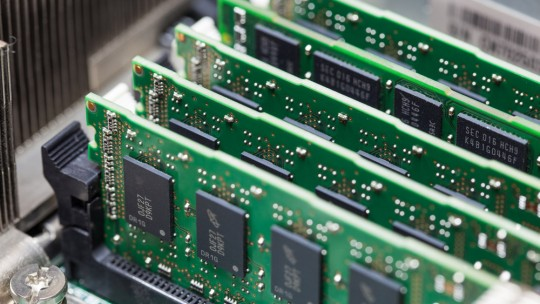
\includegraphics[width=0.5\textwidth]{figures/ram.jpg}}
\caption{RAM}
\label{ram}
\end{figure}

Selain menyimpan data tidak lenyap, simpan juga ke disk tujuan untuk mengosongkan RAM agar tidak cepat penuh.
Dalam sistem ini kita juga dapat melihat bahwa sistem operasi terletak berdekatan dengan program lain dalam RAM sehingga kemungkinan sistem operasi terganggu atau diubah oleh proses yang berjalan sangat sangat besar. Seharusnya tidak terjadi.Untuk dapat  mencegah terganggunya sistem operasi tersebut maka alamat yang tertinggi dari sistem operasi yang diletakkan pada register batas dalam CPU tersebut. Jika ada proses yang mengacu ke alamat itu atau yang lebih rendah dari itu maka proses tersebut akan di hentikan dan program tersebut akan menampilkan pesan kesalahan yang terjadi. Manajemen Memory  Untuk Multiprogramming
\begin{enumerate}
\item Pemisahan ruang-ruang alamat.
\item Pemakaian bersama memori.
\end{enumerate}

Manajer memori harus menerapkan isolasi ruang alamat dari setiap proses untuk memungkinkan proses atau proses yang diperlukan untuk mengakses. Manajer memori di lingkungan multiprogramming atau melakukan dua hal, yaitu:
\begin{itemize}
\item Perlindungan memori dengan isolasi ruang alamat oleh dis-joint.
\item Penggunaan memori bersama.
\end{itemize}

Menyalin proses bekerja bersama untuk mengakses area memori bersama. Ketika konsep multiprogramming, akses CPU dapat ditingkatkan. Sebuah model untuk pemantauan CPU probabilistik:
Pemanfaatan CPU = 1 - p n
Dengan:
\begin{enumerate}
\item N ada proses saat ini, memungkinkan untuk semua proses yang akan menunggu menggunakan I / O (Masalah CPU idle) sebesar pn. Fungsi n disebut gelar multiprogramming.
\item Waktu yang sangat lama
\end{enumerate}

\section {Kesimpulan}
Memori dan Manajemen Memori
Memori adalah pusat operasi pada sistem komputer modern, berfungsi sebagai tempat penyimpanan informasi untuk dikelola dan dipelihara sebaik mungkin. Memori adalah array besar kata atau byte, yang disebut alamat. CPU mengambil instruksi dari memori berdasarkan nilai program counter (Ama, 2003).
Sedangkan manajemen memori adalah kegiatan untuk mengatur memori komputer. Proses ini menyediakan cara untuk mengalokasikan memori untuk memproses atas permintaan mereka, membebaskannya untuk digunakan kembali ketika tidak lagi diperlukan dan mempertahankan alokasi ruang memori untuk proses tersebut. Manajemen Memori adalah salah satu bagian terpenting dari sistem operasi. pada awalnya komputer  digunakan untuk keperluan hal komputasi, kebutuhan akan memori yang lebih besar daripada kondisi fisik memori dalam sistem yang terus menerus meningkat. Dalam berbagai perhitungan dan strategi terus menerus dilakukan perbaikan untuk mengatasi keterbatasan ukuran memori fisik (Ama, 2003).
Strategi Manajemen Memori
Strategi yang dikenal sebagai berikut adalah untuk mengatasi permaslahan memori virtual. Memori virtual menyebabkan sistem seperti memiliki lebih banyak memori daripada keadaan memori fisik yang sebenarnya. Selain itu memori virtual juga tidak hanya menyediakan peningkatan komputasi.
Ruang Alamat Logis dan Fisik
Tujuan utama manajemen memori adalah konsep meletakkan ruang alamat logis ke ruang alamat fisik. Alamat logika adalah alamat yang dihasilkan didalam CPU, juga disebut dengan alamat virtual. Alamat fisik adalah alamat yang dapat terlihat oleh memori.
Swapping
Suatu proses yang harus di dalam memori sebelum dieksekusi. Proses pertukaran pertukaran keluar sementara dari memori sementara ke penyimpanan sementara dengan proses lain yang membutuhkan alokasi memori ganda untuk eksekusi.Memori penyimpanan sementara ini biasanya berupa hard disk dengan kapasitas yang bisa menampung salinan-salinan gambar memori serta menyediakan akses langsung ke gambar.